
Many models have been tested in order to compare different solutions and find the best fit for this task. This section provides a comparison between the performance of each neural network model.

Each model comes with a description of its shape (i.e. number of layers, units per layer etc.), the training history (loss and accuracy in each epoch) and the final results on the test set (confusion matrix).

%-------
\subsection{Train-Test Splitting}
\label{subsec:traintest}

The NSL-KDD dataset is already divided into a train set containing 125973 instances ($\approx 85\%$) and test set containing 22544 instances ($\approx 15\%$). We also use 15\% of the train set as \textit{dev} set, to keep track of the accuracy and loss of each model during the training phase.

The initial batch of models have been tested on the provided test set, according to the initial division. Nevertheless, during the the development of this work it was been noted that reshuffling the train and test set significantly improves the ANN performance: these results are given in Section~\ref{subsec:porcata} .

The data normalization has not been performed on the entire dataset, but separately for the train and the test set using a normalization algorithm that was fitted on the train set. This ensures that the training of the model is not affected by the values that are in the test set.

%-------
\subsection{Evaluation Metrics}
\label{subsec:traintest}

The most common evaluation metrics for IDS, as reported by \cite{nslkdd2}, are \textit{Attack Detection Rate (DR)} and \textit{False Alarm Rate (FAR)}.

$$DR = \frac{TP}{TP+FN}$$

$$FAR = \frac{FP}{FP+TN}$$

We can calculate these metrics from the confusion matrix, which is represented by the following terms.

\begin{itemize}
    \item True Positive (TP): the instance is correctly predicted as an attack.
    \item True Negative (TN): correctly predicted as a non-attack or normal instance.
    \item False Positive (FP): a normal instance is wrongly predicted as attacks. 
    \item False Negative (FN): an actual attack is wrongly predicted as non-attacks or normal instance.
\end{itemize}

False positives where a normal network activity is classified as an attack can waste the valuable time of security administrators. False negatives on the other hand have the worst impact on organizations, since an attack is not detected at all.

%-------
\subsection{All features}

Six different models where tested using all 122 features as inputs: 4 with only one hidden layer and 2 with 2 hidden layers. Table~\ref{tab:allfeat} reports the evaluation of each model.

\begin{figure}[h]
\center
  \begin{subfigure}[b]{0.6\columnwidth}
    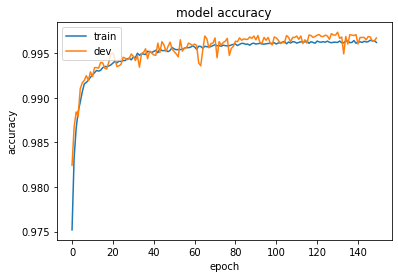
\includegraphics[width=\linewidth]{img/learn1.png}
  \end{subfigure}
  \hfill %%
  \begin{subfigure}[b]{0.6\columnwidth}
    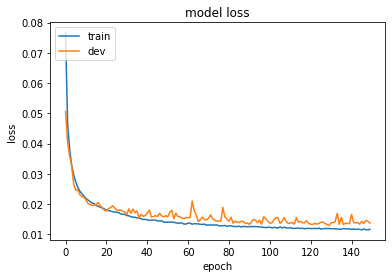
\includegraphics[width=\linewidth]{img/learn2.png}

  \end{subfigure}

      \caption{Learning Curve models of the best model trained on the full data set}
\end{figure}

\begin{table}[h]
\center
\begin{tabular}{|l|l|l||l|l|}
\hline
\multicolumn{3}{|c||}{\textbf{Model}}                                   & \multicolumn{2}{c|}{\textbf{Evaluation}} \\ \hline
\textit{Inputs} & \textit{Selection Algorithm} & \textit{Hidden Units} & \textit{DR}    & \textit{FAR}    \\ \hline
122             & None                         & 80                    &   71.4\%                  &    0.3\%                \\ \hline
122             & None                         & 80, 30                &   68.1\%                 &     0.3\%               \\ \hline
122             & None                         & 30                    &  71.92\%                   &  8.2\%                  \\ \hline
122             & None                         & 50, 10                &   72.61\%                   &   7.6\%                   \\ \hline
122             & None                         & 20                &    67.71\%                 &       7.9\%             \\ \hline
122             & None                         & 10                &    66.89\%                 &     7.7\%               \\ \hline
\end{tabular}
\caption{Comparison between models trained on the full data set}
\label{tab:allfeat}
\end{table}


%-------
\subsection{ExtraTree selected features}

Four different models where tested using ExtraTree Classifier as feature selection algorithm: 2 with the top 80 features and 2 with the top 15 features in the importance ranking. Table~\ref{tab:treefeat} reports the evaluation of each model.


\begin{table}[h]
\center
\begin{tabular}{|l|l|l||l|l|}
\hline
\multicolumn{3}{|c||}{\textbf{Model}}                                   & \multicolumn{2}{c|}{\textbf{Evaluation}} \\ \hline
\textit{Inputs} & \textit{Selection Algorithm} & \textit{Hidden Units} & \textit{DR}    & \textit{FAR}    \\ \hline
80             & ExtraTree                         & 10                    &   61.1\%                  &   7.8\%                 \\ \hline
80             & ExtraTree                         & 30, 10               &   69.29\%                  &    7.6\%                \\ \hline
40             & ExtraTree                         & 10                    &   59.7\%                  &   3\%                 \\ \hline
40             & ExtraTree                         & 30, 10               &   59.5\%                  &     3\%               \\ \hline
15             & ExtraTree                         & 8                &       67.2\%              &   6.86\%                 \\ \hline
15             & ExtraTree                         & 4                &       64.6\%              &   7.3\%                 \\ \hline
\end{tabular}
\caption{Comparison between models trained on ExtraTree selecte features}
\label{tab:treefeat}
\end{table}

%%%%

\begin{figure}[h]
\center
  \begin{subfigure}[b]{0.6\columnwidth}
    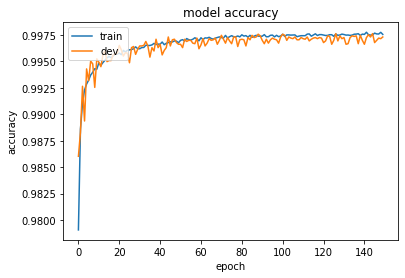
\includegraphics[width=\linewidth]{img/learn3.png}
  \end{subfigure}
  \hfill %%
  \begin{subfigure}[b]{0.6\columnwidth}
 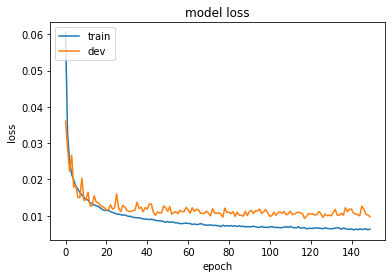
\includegraphics[width=\linewidth]{img/learn4.png}
  \end{subfigure}
\caption{Learning Curve models of the best model trained on Extra Tree selected features}
\end{figure}

%-------
\subsection{Univariate selected features}

Four different models where tested using Univariate Selection as feature selection algorithm: 2 with the top 80 features and 2 with the top 15 features in the importance ranking. Table~\ref{tab:univfeat} reports the evaluation of each model.

\begin{table}[h]
\center
\begin{tabular}{|l|l|l||l|l|}
\hline
\multicolumn{3}{|c||}{\textbf{Model}}                                   & \multicolumn{2}{c|}{\textbf{Evaluation}} \\ \hline
\textit{Inputs} & \textit{Selection Algorithm} & \textit{Hidden Units} & \textit{DR}    & \textit{FAR}    \\ \hline
80             & Univariate                         & 10                    &   66.56\%                  &   7.4\%                 \\ \hline
80             & Univariate                         & 30, 10               &     70\%                &   7.4\%                 \\ \hline
40             & Univariate                         & 10                    &    69\%                 &   7.8\%                 \\ \hline
40             & Univariate                         & 30, 10               &   73.7\%                  &    3.4\%                \\ \hline
15             & Univariate                         & 8                &    57\%                 &      7.4\%              \\ \hline
15             & Univariate                         & 4                &    63.7\%                 &          3.1\%          \\ \hline
\end{tabular}
\caption{Comparison between models trained on Univariate selected features}
\label{tab:univfeat}
\end{table}

%%%%

\begin{figure}[h]
\center
  \begin{subfigure}[b]{0.6\columnwidth}
    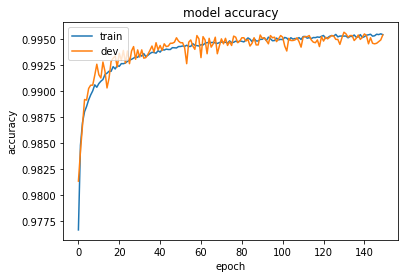
\includegraphics[width=\linewidth]{img/learn5.png}
  \end{subfigure}
  \hfill %%
  \begin{subfigure}[b]{0.6\columnwidth}
 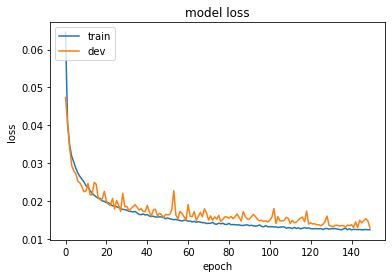
\includegraphics[width=\linewidth]{img/learn6.png}
  \end{subfigure}
\caption{Learning Curve models of the best model trained on Univariate selected features}
\end{figure}


%-------
\subsection{Re-shuffled Train Set}
\label{subsec:porcata}

Given that the results of the preceding models are far from being enough to deploy an IDS in a real network, another approach has been tried. The train and test set have been merged together, split again in train and test set and re-normalized using a normalization based on the train set alone. This approach gave much better results, meaning that probably the test set has many outliers that have to be taken into account when designing the ANN. Figure~\ref{tab:porcata} displays the results of the same models but with the shuffled dataset.

\begin{figure}[h]
\center
  \begin{subfigure}[b]{0.6\columnwidth}
    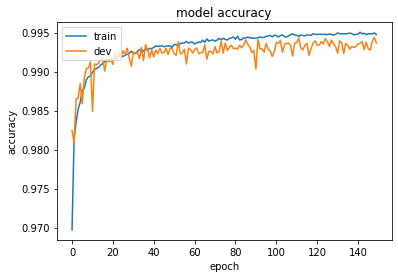
\includegraphics[width=\linewidth]{img/learn7.png}
  \end{subfigure}
  \hfill %%
  \begin{subfigure}[b]{0.6\columnwidth}
 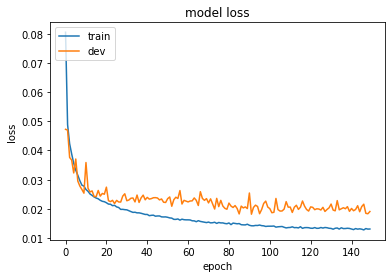
\includegraphics[width=\linewidth]{img/learn8.png}
  \end{subfigure}
\caption{Learning Curve models of the best model trained on the shuffled data set}
\end{figure}

\begin{table}[h]
\center
\begin{tabular}{|l|l|l||l|l|}
\hline
\multicolumn{3}{|c||}{\textbf{Model}}                                   & \multicolumn{2}{c|}{\textbf{Evaluation}} \\ \hline
\textit{Inputs} & \textit{Selection Algorithm} & \textit{Hidden Units} & \textit{DR}    & \textit{FAR}    \\ \hline
122             & None                         & 10                    &   99.18\%                  &   1.2\%                 \\ \hline
122             & None                         & 50, 10               &     99\%                &  0.6\%                 \\ \hline
122             & None                         & 20                    &    98.15\%                 &   0.3\%                 \\ \hline
122             & None                         & 30                    &    99.3\%                 &   0.8\%                 \\ \hline
122             & None                         & 80, 30               &   99.3\%                  &    0.5\%                \\ \hline  \hline
80             & Univariate                         & 10                    &   98.6\%                  &   1.8\%                 \\ \hline
80             & Univariate                         & 30, 10               &     99\%                &   1.1\%                 \\ \hline
40             & Univariate                         & 10                    &    98.18\%                 &   1.8\%                 \\ \hline
40             & Univariate                         & 30, 10               &   98.7\%                  &    1.3\%                \\ \hline
15             & Univariate                         & 8                &    90.9\%                 &      3.2\%              \\ \hline
15             & Univariate                         & 4                &    91.6\%                 &          3.7\%          \\ \hline
\end{tabular}
\caption{DR and FAR with new train/test set splitting}
\label{tab:porcata}
\end{table}